\section{\secstdgraphs}
\label{sec_std_graphs}

As we have seen, graphs can model many different situations. The drawing of a graph may lead to insights about the problem the graph is modeling.  But the true power of graph models comes from a well-developed theory of graphs-- facts that are true about all graphs, and the ability to implement algorithms on graphs using computer tools.  We begin this section with some theory, the first theorem of graph theory. Next, graphs often have standard pieces, such as a row of connected vertices (a path), a circle of connected vertices (a cycle), or even a group of vertices that are all adjacent to each other (a complete graph).  We introduce these and other standard graphs.  To implement algorithms on a graph, we first need to enter the graph into a computer program. We introduce one such tool, the adjacency matrix of a graph. 

%%%%%%%%%%%%%%%%%%%%%%%%%%%%%%%%%%

\newcommand{\subdegseq}{Degree Sequences}
\subsection{\subdegseq}
\label{sub_degree_seq}

One characteristic of a graph is the list of degrees of all the vertices.  Some algorithms that run on graphs require a certain smallest or largest degree, or even that all the vertices have the same degrees.  We define a few relevant terms.

\begin{defn}[Degree sequence and regular graphs]
\label{defn_ds_regular} 
~
    \begin{apart}
        \item The \vocab{degree sequence} of a graph is a list of the degrees of the vertices, including multiplicities.  The degree sequence is usually written in nonincreasing order, which means largest to smallest. For example, the degree sequence of the classmates graph drawn in \Cref{fig_classmates_graph} is 
            $$3, 3, 3, 2, 1, 0.$$

        \item It is possible that all the vertices of a graph have the same degree.  A graph is \vocab{regular} if all its vertices have the same degree.  A regular graph is $r$-\vocab{regular} if every vertex has degree $r$.  For example, the graph in \Cref{fig_4reg} is regular because every vertex has degree four.  
    \end{apart}

        \begin{figure}[hbtp]
            \centering
            %Used in \Cref{sec_subgraph_isomorphic}.

\begin{tikzpicture}
[scale =.55, auto=left]
\GraphInit[vstyle=Welsh]
\SetGraphUnit{1.6}
\SetVertexNoLabel
\Vertices{circle}{$y$, $z$,$a$,$u$, $v$,$w$,$x$}
\Edges($a$,$u$,$v$,$w$,$x$,$y$,  $z$,$a$)
\Edges($a$,$v$,$x$,$z$,$u$,$w$,  $y$,$a$)
\end{tikzpicture}
            \caption{A 4-regular graph ($H_{4,6}$).}
            \label{fig_4reg}
        \end{figure}
\end{defn}

Try working with these definitions.

\begin{act}[Degrees]
\label{act_deg_seq}
    Consider the graph $S$ drawn in \Cref{fig_act_deg_seq}.

    \begin{figure}
        \centering
        %Used in \Cref{sec_graph_thy}.

\begin{tikzpicture}
[scale =.5]
\GraphInit[vstyle=Welsh]
\SetGraphUnit{1.6}
%\SetVertexNoLabel
\Vertices{circle}{$c$,$b$, $a$, $f$,$e$, $d$}
\Edges($a$, $b$, $c$, $d$, $e$,$a$)
\Edges($c$,$f$)
\Edges($e$,$b$,$d$)
\end{tikzpicture}
        \caption{A graph $S$ of order six.}
        \label{fig_act_deg_seq}
    \end{figure}
   
    \begin{apart}
        \item Find the degree sequence of $S$.
        \item Is $S$ regular?
        \item Calculate the sum of the degrees of the vertices in $S$.
        \item \label{part_degree_sum} How is the sum of the degrees of the vertices related to the number of edges in $S$? Can you explain why? 
        \item Draw a new 3-regular graph with six vertices.
        \item \label{part_3reg_order5} Can you draw a 3-regular graph with five vertices?  Explain.
    \end{apart}
\end{act}

In \Cref{act_deg_seq} (\ref{part_degree_sum}), we observed a relationship between the degree sequence of $S$ and the number of edges in $S$: if we add up the degrees of all the vertices in a graph, then we count each edge of the graph twice, because each endpoint of an edge counts that edge as part of their degree.  

Perhaps this discussion reminds you of the Handshakes Puzzle (\Cref{act_handshakes}). If each person reports the number of handshakes they did and we calculate the sum, then we count each handshake twice. Therefore, that sum would be twice the number of handshakes. 

We state the general observation as a theorem. 

\begin{thm}[The first theorem of graph theory]
\label{thm_first_thm_graph_thy}
    The sum of the degrees of the vertices of a graph, counting multiplicities, is twice the number of edges.  Equivalently, the number of edges of a graph is half of the sum of the degrees of the vertices. 
\end{thm}

One benefit of this theorem is that visually counting edges in a complicated graph can be a challenge, but counting degrees is often easier. 

Let's practice using this theorem.

\begin{exam}[Checking first theorem of graph theory]
\label{exam_check_first_thm_graph_thy}
~
    \begin{apart} 
        \item Check \Cref{thm_first_thm_graph_thy} for the classmates graph drawn in \Cref{fig_classmates_graph}.
            \begin{soln}
                The sum of the degrees is 
                    $$3+3+3+2+1+0 = 12.$$             
                The number of edges is $\frac{12}{2}=6$, as expected.
            \end{soln}
        \item In \Cref{act_deg_seq} (\ref{part_3reg_order5}), we considered whether there exists a 3-regular graph of order five.  Use \Cref{thm_first_thm_graph_thy} to explain why there cannot exist such a graph.
            \begin{soln}
                If there were such a graph, then the sum of the degrees would be $$3+3+3+3+3 = 15$$ which is an odd integer but, by \Cref{thm_first_thm_graph_thy}, the sum of the degrees is twice the number of edges, which is an even integer.  Since an integer cannot be even and odd (which we will formally prove in \Cref{thm_div_alg}), such a graph is impossible.  %By the way, we are using a proof by contradiction (\Cref{pff_contradiction}).
            \end{soln}  
        \end{apart}
\end{exam}

It is interesting to ask if a given list of nonnegative integers is the degree sequence of a graph.

\begin{exam}[Is this list a degree sequence of a graph?]
\label{exam_graphical}
   For each list of nonnegative integers, draw a graph with that degree sequence or explain why there cannot be a graph with that degree sequence.
       \begin{apart}
           \item $5, 5, 3, 3, 3, 3$
               \begin{soln}
                   Let's see what happens if we can draw a graph with this degree sequence.  Note that there are six numbers listed, so our graph has six vertices.  Therefore, each of the degree five vertices must be adjacent to all of the other five vertices.  Therefore, our graph must start as shown on the left in \Cref{fig_graphical}.  The vertices $v_2$ and $w_2$ have degree five, but the other vertices only have degree two.  We can increase their degree to three, as desired, by adding the edges $\{v_1,w_1\}$ and $\{v_3,w_3\}$, for example, obtaining the graph drawn on the right in \Cref{fig_graphical}.  Thus, this list is the degree sequence of a graph.
                       \begin{figure}[htbp]
                           \centering
                           %Used in \Cref{sec_graph_thy}, \Cref{exam_graphical}.
% Note:  full graph is graphical_finish

%% STARTING ATTEMPT
\begin{tikzpicture}
    [scale =.75]
    \GraphInit[vstyle=Welsh]
    \SetGraphUnit{2}
        %\SetVertexNoLabel
    % bottom row
    \Vertex[LabelOut,Lpos=-90,x=0,y=0]{$w_1$}
    \Vertex[LabelOut,Lpos=-90,x=1.5,y=0]{$w_2$} 
    \Vertex[LabelOut,Lpos=-90,x=3,y=0]{$w_3$}
    \Edges($w_1$,$w_2$,$w_3$)
    % top row
    \Vertex[LabelOut,Lpos=90,x=0,y=1.5]{$v_1$}
    \Vertex[LabelOut,Lpos=90,x=1.5,y=1.5]{$v_2$} 
    \Vertex[LabelOut,Lpos=90,x=3,y=1.5]{$v_3$}
    \Edges($v_1$,$v_2$,$v_3$)
    % vertical edges
    %\Edges($v_1$,$w_1$)
    \Edges($v_2$,$w_2$)
    %\Edges($v_3$,$w_3$)
    % the rest of the Xs
    \Edges($v_1$,$w_2$,$v_3$)
    \Edges($w_1$,$v_2$,$w_3$)
\end{tikzpicture}
\hspace{1 in}
%% COMPLETED VERSION
\begin{tikzpicture}
    [scale =.75]
    \GraphInit[vstyle=Welsh]
    \SetGraphUnit{2}
        %\SetVertexNoLabel
    % bottom row
    \Vertex[LabelOut,Lpos=-90,x=0,y=0]{$w_1$}
    \Vertex[LabelOut,Lpos=-90,x=1.5,y=0]{$w_2$} 
    \Vertex[LabelOut,Lpos=-90,x=3,y=0]{$w_3$}
    \Edges($w_1$,$w_2$,$w_3$)
    % top row
    \Vertex[LabelOut,Lpos=90,x=0,y=1.5]{$v_1$}
    \Vertex[LabelOut,Lpos=90,x=1.5,y=1.5]{$v_2$} 
    \Vertex[LabelOut,Lpos=90,x=3,y=1.5]{$v_3$}
    \Edges($v_1$,$v_2$,$v_3$)
    % vertical edges
    \Edges($v_1$,$w_1$)
    \Edges($v_2$,$w_2$)
    \Edges($v_3$,$w_3$)
    % the rest of the Xs
    \Edges($v_1$,$w_2$,$v_3$)
    \Edges($w_1$,$v_2$,$w_3$)
\end{tikzpicture}
                           \caption{Drawing a graph with degree sequence $5, 5, 3, 3, 3, 3$.}
                           \label{fig_graphical}
                        \end{figure}
                    Note that this graph is not the only graph with this degree sequence.  We could have drawn edges between $v_1$ and $v_3$ and between $w_1$ and $w_3$, for example.
               \end{soln}
            \item $5, 5, 3, 2, 2, 1$
                \begin{soln}
                    Let's see if we can draw a graph with this degree sequence.  It would have six vertices.  As before, the two vertices of degree five would each be adjacent to the other four vertices, as in the graph drawn on the left in \Cref{fig_graphical}.  But then all of the other vertices in our graph would already have degree at least two.  That is a problem because our degree sequence lists a vertex of degree one. Thus, this list is not the degree sequence of any graph.
                \end{soln}
       \end{apart}
\end{exam}

%%%%%%%%%%%%%%%%%%%%%%%%%%%%%%%%%%%

\newcommand{\substdgraphs}{Standard Graphs}
\subsection{\substdgraphs}
\label{sub_standard_graphs}

We begin our tour of some standard graphs with two different families of graphs related to handshakes.

\begin{exam} [Handshakes graphs]
\label{exam_handshake_graphs}
~     
    \begin{apart}
        \item \label{part_hs_complete} In \Cref{exam_hs6} we drew a graph representing a group of six students shaking hands with each other, as drawn again in \Cref{fig_K6_again}.  How many vertices does this graph have and what does that number mean in the story? How many edges does that graph have and what does that number mean in the story?
            \begin{soln}
                The graph has six vertices that represent the six students.  The graph has 15 edges that represent the 15 handshakes the group did.
            \end{soln}

            \begin{figure}[hbtp]
                 \centering
                 %Used in \Cref{sec_GS_CC}

    \begin{tikzpicture}
        [scale =2]
        \GraphInit[vstyle=Welsh]
        \SetGraphUnit{1}
        \SetVertexNoLabel
        \Vertices{circle}{$B$,$A$, $F$,$E$,$D$,$C$}
        \Edges($A$, $B$, $C$, $D$, $E$, $F$, $A$)
        \Edges($A$, $C$, $E$, $A$)
        \Edges($B$, $D$, $F$, $B$) 
        \Edges($A$, $D$)
        \Edges($B$, $E$)
        \Edges($C$, $F$)
    \end{tikzpicture}
                 \caption{A drawing of the complete graph $K_6$ showing six students shaking hands with each other.}
                 \label{fig_K6_again}
             \end{figure}
        \item \label{part_hs_complete_bipartite} Six discrete mathematics students had just finished shaking hands and started studying when three first-year students wandered into the room.  The discrete students thought it would be polite to greet each visitor by shaking hands.  (Each discrete mathematics student shakes hands with each first-year student.) Draw a graph representing this new situation, only including the new handshakes.
             \begin{soln}
                 We draw the graph in \Cref{fig_K6b3} and, as is common, we distinguish between the two types of students representing the discrete students with black vertices and the first-year students with white vertices.  Which group is which color is not important and we do not have to color the vertices at all.  Notice that there are $6+3=9$ vertices representing the nine students and there are $6\cdot3=18$ edges representing the 18 new handshakes.
             \end{soln}

             \begin{figure} [hbtp]
                 \centering
                 %Used in \Cref{sec_std_graphs}.

\begin{tikzpicture}
    [scale =.5]
        \GraphInit[vstyle=Welsh]
        \SetGraphUnit{2}
        \SetVertexNoLabel
        \Vertex[LabelOut,Lpos=90,x=0,y=3]{$d_1$}
        \Vertex[LabelOut,Lpos= 90,x=1.5,y=3]{$d_2$}
        \Vertex[LabelOut,Lpos=-90,x=3,y=3]{$d_3$}
        \Vertex[LabelOut,Lpos= -90,x=4.5,y=3]{$d_4$}
        \Vertex[LabelOut,Lpos= -90,x=6,y=3]{$d_5$}
        \Vertex[LabelOut,Lpos= -90,x=7.5,y=3]{$d_6$}
        \Vertex[LabelOut,Lpos=90,x=2.25,y=0]{$f_1$}
        \Vertex[LabelOut,Lpos= 90,x=3.75,y=0]{$f_2$}
        \Vertex[LabelOut,Lpos=-90,x=5.25,y=0]{$f_3$}
        \Edges($d_1$, $f_1$, $d_2$)
        \Edges($d_3$, $f_1$, $d_4$)
        \Edges($d_5$, $f_1$, $d_6$)
        \Edges($d_1$, $f_2$, $d_2$)
        \Edges($d_3$, $f_2$, $d_4$)
        \Edges($d_5$, $f_2$, $d_6$)
        \Edges($d_1$, $f_3$, $d_2$)
        \Edges($d_3$, $f_3$, $d_4$)
        \Edges($d_5$, $f_3$, $d_6$)

        \AddVertexColor{black}{$d_1$, $d_2$, $d_3$, $d_4$, $d_5$, $d_6$}
    \end{tikzpicture}
                 \caption{A drawing of the complete bipartite graph $K_{6,3}$ showing six discrete math students shaking hands with three first-year students.}
                 \label{fig_K6b3}
             \end{figure}
    \end{apart}  
\end{exam}

\Cref{exam_handshake_graphs} introduced two important families of graphs.

\begin{defn}[Complete graphs and complete bipartite graphs]
\label{defn_complete_completebipartite}
~
    \begin{apart}
        \item A \vocab{family} of graphs is a set of graphs that share many properties. We might define a family in terms of a parameter such as $s$.  In the name of the family, we often write that parameter as a \vocab{subscript}, a character written slightly smaller and lower. For example, the family of complete graphs $K_s$ (pronounced ``$K$ sub $s$'') for $n\ge1$ are the graphs $K_1$, $K_2$, $K_3$, \ldots.  
        
        \item For $s \ge 1$ the \vocab{complete graph} (or \vocab{handshake graph}) with $s$ vertices, denoted $K_s$, has an edge between every pair of vertices. The subscript $s$ tells us the number of vertices.  Note that ``complete'' starts with the sound of the letter ``K''.   For example, in \Cref{exam_handshake_graphs} (\ref{part_hs_complete}), we drew  the complete graph $K_6$. 

        \item For integers $s,t \ge 1$, the \vocab{complete bipartite graph} with $s$ vertices of the first type (perhaps colored black in the drawing) and $t$ vertices of the second type (perhaps colored white in the drawing), denoted $K_{s,t}$ has an edge between each vertex of the first type and each vertex of the second type (and no other edges). For example, in \Cref{exam_handshake_graphs} (\ref{part_hs_complete_bipartite}), we drew the complete bipartite graph $K_{6,3}$.   
        \item A special case of complete bipartite graphs is the \vocab{star} graphs $K_{1,t}$ for $t\ge1$.  For example, a star graph might model a corporate reporting structure such as a vice-president and their directors. \Cref{fig_stars_K1b4_K1b5} shows drawings of $K_{1,4}$ and $K_{1,5}$ where we have drawn the white vertices in a circle around the central black \vocab{hub} vertex, as is customary. 
        
            \begin{figure}[ht]
                \centering            %Used in \Cref{sec_graph_models}.

% Star K_1,4
\begin{tikzpicture}
[scale =.5]
\GraphInit[vstyle=Welsh]
\SetGraphUnit{2}
\SetVertexNoLabel
\Vertices{circle}{$B$,$A$,$D$,$C$}
\Vertex[LabelOut,Lpos= -90,x=0,y=0]{$Z$}
\Edges($A$, $Z$, $C$)
\Edges($B$, $Z$, $D$)
\AddVertexColor{black}{$Z$}
\end{tikzpicture}
%
\hspace{.35in} %%%%
%
% Star K_1,5
\begin{tikzpicture}
[scale =.5]
\GraphInit[vstyle=Welsh]
\SetGraphUnit{2}
\SetVertexNoLabel
\Vertices{circle}{$B$,$A$,$E$,$D$,$C$}
\Vertex[LabelOut,Lpos= -90,x=0,y=0]{$Z$}
\Edges($A$, $Z$, $C$)
\Edges($B$, $Z$, $D$)
\Edges($Z$, $E$)
\AddVertexColor{black}{$Z$}
\end{tikzpicture}

                \caption{The stars $K_{1,4}$ and $K_{1,5}$.}                \label{fig_stars_K1b4_K1b5}
            \end{figure}        
    \end{apart}   
\end{defn}

Let's look more closely at a few examples.

\begin{exam}[Complete, complete bipartite, and star graphs]
\label{exam_complete_completebipartite_star}
~    
        \begin{apart}
            \item Draw the complete graphs $K_1$, $K_2$, $K_3$, $K_4$, and $K_5$.
                \begin{soln}
                    See \Cref{fig_complete_graphs_12345}.
                \end{soln}

                \begin{figure} [hbtp]
                    \centering
                     %Used in \Cref{sec_graph_models}       
 
% K1
     \begin{tikzpicture}
        [scale =.5]
        \GraphInit[vstyle=Welsh]
        \SetGraphUnit{2}
        \SetVertexNoLabel
    
        \Vertex[LabelOut,Lpos=90,x=0,y=0]{$A$}
    \end{tikzpicture}
\hspace{.35in} %%%
% K2
    \begin{tikzpicture}
        [scale =.5]
        \GraphInit[vstyle=Welsh]
        \SetGraphUnit{2}
        \SetVertexNoLabel
        \Vertex[LabelOut,Lpos=90,x=0,y=0]{$A$}
        \Vertex[LabelOut,Lpos= 90,x=3,y=0]{$B$}
        \Edges($A$, $B$)
    \end{tikzpicture}
\hspace{.35in} %%%
% K3
    \begin{tikzpicture}
        [scale =.5]
        \GraphInit[vstyle=Welsh]
        \SetGraphUnit{2}
        \SetVertexNoLabel
        \Vertices{circle}{$B$,$A$,$C$}
        \Edges($A$, $B$, $C$, $A$)
    \end{tikzpicture}
\hspace{.35in} %%%
% K4
    \begin{tikzpicture}
        [scale =.5]
        \GraphInit[vstyle=Welsh]
        \SetGraphUnit{2}
        \SetVertexNoLabel
        \Vertices{circle}{$B$,$A$,$D$,$C$}
        \Edges($A$, $B$, $C$, $D$, $A$)
        \Edges($A$, $C$)
        \Edges($B$, $D$)
    \end{tikzpicture}
\hspace{.35in} %%%
% K5
    \begin{tikzpicture}
        [scale =.5]
        \GraphInit[vstyle=Welsh]
        \SetGraphUnit{2}
        \SetVertexNoLabel
        \Vertices{circle}{$B$,$A$,$E$,$D$,$C$}
        \Edges($A$, $B$, $C$, $D$, $E$, $A$)
        \Edges($A$, $C$, $E$, $B$, $D$, $A$)
    \end{tikzpicture}
                    \caption{The complete graphs $K_1$, $K_2$, $K_3$, $K_4$, and $K_5$.}
                    \label{fig_complete_graphs_12345}
                \end{figure}
        
            \item For each graph, count the number of vertices and edges and determine the degree sequence: the complete graph $K_6$, the complete bipartite graph $K_{6,3}$, and the star $K_{1,5}$

                \begin{soln}
                    The complete graph $K_6$ has six vertices and 15 edges. Every vertex has degree five, and so the degree sequence is $5,5,5,5,5,5$.
                    
                    The complete bipartite graph $K_{6,3}$ has nine vertices and 18 edges.  The black vertices have degree three and the white vertices have degree six, so the degree sequence is $6,6,6,3,3,3,3,3,3$.

                    The star graph $K_{1,5}$ has six vertices and five edges. Its hub vertex has degree five and the end vertices have degree one, so its degree sequence is $5,1,1,1,1,1$.
                \end{soln}

            \item Draw the complete bipartite graph $K_{4,4}$.    
                \begin{soln}
                    See \Cref{fig_K4b4}.
                \end{soln}

                \begin{figure}[hbtp]
                    \centering
                    %Used in \Cref{sec_std_graphs}.

\begin{tikzpicture}
    [scale =.5]
        \GraphInit[vstyle=Welsh]
        \SetGraphUnit{2}
        \SetVertexNoLabel
        \Vertex[LabelOut,Lpos=90,x=0,y=3]{$d_1$}
        \Vertex[LabelOut,Lpos= 90,x=1.5,y=3]{$d_2$}
        \Vertex[LabelOut,Lpos=-90,x=3,y=3]{$d_3$}
        \Vertex[LabelOut,Lpos= -90,x=4.5,y=3]{$d_4$}
        \Vertex[LabelOut,Lpos=90,x=0,y=0]{$f_1$}
        \Vertex[LabelOut,Lpos= 90,x=1.5,y=0]{$f_2$}
        \Vertex[LabelOut,Lpos=-90,x=3,y=0]{$f_3$}
        \Vertex[LabelOut,Lpos=-90,x=4.5,y=0]{$f_4$}

        
        \Edges($d_1$, $f_1$, $d_2$)
        \Edges($d_3$, $f_1$, $d_4$)

        \Edges($d_1$, $f_2$, $d_2$)
        \Edges($d_3$, $f_2$, $d_4$)

        \Edges($d_1$, $f_3$, $d_2$)
        \Edges($d_3$, $f_3$, $d_4$)

        \Edges($d_1$, $f_4$, $d_2$)
        \Edges($d_3$, $f_4$, $d_4$)
        
        \AddVertexColor{black}{$d_1$, $d_2$, $d_3$, $d_4$}
    \end{tikzpicture}
                    \caption{The complete bipartite graph $K_{4,4}$}
                    \label{fig_K4b4}
                \end{figure}
        \end{apart}
\end{exam}

There are two more important families of graphs.

\begin{defn}[Paths and cycles]
\label{defn_paths_cycles}
~
    \begin{apart}
        \item For $s \ge 1$, the \vocab{path} with $s$ vertices, denoted $P_s$, has $s$ vertices each adjacent to the next in a row.  Officially, if the vertex set is $\{v_1, v_2, \ldots, v_s\}$, then the edge set is $$\{\{v_1,v_2\}, \{v_2,v_3,\}, \ldots, \{v_{s-1},v_s\}\}.$$  For example, \Cref{fig_P4_P5} shows drawings of the paths $P_4$ and $P_5$.
            \begin{figure}[ht]
                \centering
                %Used in \Cref{sec_graph_models}.
\begin{tikzpicture}
    [scale =.5]
    \GraphInit[vstyle=Welsh]
    \SetGraphUnit{2}
    \SetVertexNoLabel
% P4
    \Vertex[LabelOut,Lpos=90,x=0,y=0]{a}
    \Vertex[LabelOut,Lpos=90,x=1.5,y=0]{b} 
    \Vertex[LabelOut,Lpos=90,x=3,y=0]{c}
    \Vertex[LabelOut,Lpos=90,x=4.5,y=0]{d}
    \Edges(a,b,c,d)
\end{tikzpicture}
%
\hspace{.35in} %%%%
%
\begin{tikzpicture}
    [scale =.5]
    \GraphInit[vstyle=Welsh]
    \SetGraphUnit{2}
    \SetVertexNoLabel
% P5
    \Vertex[LabelOut,Lpos=90,x=0,y=0]{A}
    \Vertex[LabelOut,Lpos=90,x=1.5,y=0]{B} 
    \Vertex[LabelOut,Lpos=90,x=3,y=0]{C}
    \Vertex[LabelOut,Lpos=90,x=4.5,y=0]{D}    
    \Vertex[LabelOut,Lpos=90,x=6,y=0]{E}
    \Edges(A,B,C,D,E)
\end{tikzpicture}
                \caption{The paths $P_4$ and $P_5$.}
                \label{fig_P4_P5}
            \end{figure}
        
        \item For $s \ge 3$, the \vocab{cycle} with $s$ vertices, denoted $C_s$, has $s$ vertices each adjacent to the next in a circle.  Officially, if the vertex set is $\{v_1, v_2, \ldots, v_s\}$, then the edge set is $$\{\{v_1,v_2\}, \{v_2,v_3,\}, \ldots, \{v_{s-1},v_s\},\{v_s,v_1\}\}.$$ For example, \Cref{fig_C4_C5} shows drawings of the cycles $C_4$ and $C_5$.
            \begin{figure}[htbp]
                \centering
                %Used in \Cref{sec_graph_models}.
\begin{tikzpicture}
    [scale =.5]
    \GraphInit[vstyle=Welsh]
    \SetGraphUnit{2}
    \SetVertexNoLabel
% C4
    \Vertices{circle}{a,b,c,d}
    \Edges(a,b,c,d,a)
\end{tikzpicture}
%
\hspace{.35in} %%%%
%
\begin{tikzpicture}
    [scale =.5]
    \GraphInit[vstyle=Welsh]
    \SetGraphUnit{2}
    \SetVertexNoLabel
% C5
    \Vertices{circle}{a,b,c,d,e}
    \Edges(a,b,c,d,e,a)
\end{tikzpicture}
                \caption{The cycles $C_4$ and $C_5$.}
                \label{fig_C4_C5}
            \end{figure}
    \end{apart}    
\end{defn}

Let's look at an example.

\begin{exam}[Paths and cycles]
\label{exam_paths_cycles}
    For each graph, count the number of vertices and edges and write the degree sequence.
        \begin{apart}
            \item The paths $P_4$ and $P_5$.
                \begin{soln}
                    The path $P_4$ has four vertices and three edges.  The end vertices have degree one and the middle vertices have degree two.  The degree sequence is $2,2,1,1$. 

                    The path $P_5$ has five vertices and four edges.  The degree sequence is $2,2,2,1,1$. 
                \end{soln}
            \item The cycles $C_4$ and $C_5$.
                \begin{soln}
                    The cycle $C_4$ has four vertices and four edges.  Every vertex has degree two, and so the degree sequence is $2,2,2,2$.

                    The cycle $C_5$ has five vertices, five edges, and degree sequence $2,2,2,2,2$.
                \end{soln} 
        \end{apart}
\end{exam}

Practice working with standard graphs and reading new definitions for families of graphs.

\begin{act}[Standard families of graphs]
\label{act_std_families}
    Draw each graph, count the number of vertices and edges, and list the degree sequence.  
~
    \begin{apart}
        \item The complete graph $K_4$.       
        \item The complete bipartite graph $K_{2,5}$.
        \item The star $K_{1,6}$.
        \item The path $P_3$.
        \item The cycle $C_6$.
        
        \item \label{part_wheel} The wheel $W_5$ consists of the cycle $C_5$ with an additional hub vertex that is adjacent to each vertex in the cycle. 
        
        \item \label{part_ladder} The ladder $L_{2\times5}$ consists of two copies of the path $P_5$ with $5$ additional edges between each pair of corresponding vertices.  Officially, if the vertex set is $\{v_1,v_2,v_3,v_4,v_5,,w_1,w_2,w_3,w_4,w_5\}$, then the edges are
        
            \begin{center}
            \begin{tabular}{ll}
               top rail: & $\{v_1,v_2\}, \{v_2,v_3\}, \{v_3,v_4\}, \{v_4,v_5\}$ \\
               bottom rail: & $\{w_1,w_2\}, \{w_2,w_3\}, \{w_3,w_4\},\{w_4,w_5\}$ \\
               rungs: & $\{v_1,w_1\}, \{v_2,w_2\}, \{v_3,w_3\},\{v_4,w_4\}, \{v_5,w_5\}.$
            \end{tabular}
            \end{center}
    \end{apart}
\end{act}

Let's check answers to \Cref{act_std_families} (\ref{part_wheel}) and (\ref{part_ladder}). We begin with a definition.

\begin{defn}[Wheels and ladders]
\label{defn_wheel_ladder}
~
    \begin{apart}
        \item For $s \ge 3$, the \vocab{wheel}, denoted $W_s$, consists of the cycle $C_s$ with an additional \vocab{hub} vertex that is adjacent to each vertex in the cycle. For example, \Cref{fig_W3} shows a drawing of $W_3$.
            \begin{figure}[hbtp]
                \centering
                %Used in \Cref{sec_std_graphs}.

\begin{tikzpicture}
    [scale =.5]
    \GraphInit[vstyle=Welsh]
    \SetGraphUnit{2}
    \SetVertexNoLabel
% W3
    \Vertices{circle}{a,b,c}
    \Vertex[x=0,y=0]{z}
    \Edges(a,b,c,a)
    \Edges(a,z,b)
    \Edges(c,z)
\end{tikzpicture}

                \caption{The wheel $W_3$.}
                \label{fig_W3}
            \end{figure}
        
        \item For $t \ge 1$, \vocab{ladder}, denoted $L_{2\times t}$, consists of two copies of the path $P_t$ with $t$ additional edges between each pair of corresponding vertices.  Officially, if the vertex set is $\{v_1,v_2,\ldots,v_t,w_1,w_2,\ldots,w_t\}$, then the edges are
        
            \begin{center}
            \begin{tabular}{ll}
               top rail: & $\{v_1,v_2\}, \{v_2,v_3\}, \ldots, \{v_{t-1},v_t\}$ \\
               bottom rail: & $\{w_1,w_2\}, \{w_2,w_3\}, \ldots, \{w_{t-1},w_t\}$ \\
               rungs: & $\{v_1,w_1\}, \{v_2,w_2\}, \ldots, \{v_t,w_t\}.$
            \end{tabular}
            \end{center}
        For example, \Cref{fig_L2x4} shows a drawing of $L_{2 \times 4}$.
            \begin{figure}[hbtp]
                \centering
                %Used in \Cref{sec_std_graphs}.
% Ladder = Lattice $L_{2 \times 4}$$

\begin{tikzpicture}
    [scale =.75]
    \GraphInit[vstyle=Welsh]
    \SetGraphUnit{2}
        %\SetVertexNoLabel
    % bottom row
    \Vertex[LabelOut,Lpos=-90,x=0,y=0]{$w_1$}
    \Vertex[LabelOut,Lpos=-90,x=1.5,y=0]{$w_2$} 
    \Vertex[LabelOut,Lpos=-90,x=3,y=0]{$w_3$}
    \Vertex[LabelOut,Lpos=-90,x=4.5,y=0]{$w_4$}    
    \Edges($w_1$,$w_2$,$w_3$,$w_4$)
    % top row
    \Vertex[LabelOut,Lpos=90,x=0,y=1.5]{$v_1$}
    \Vertex[LabelOut,Lpos=90,x=1.5,y=1.5]{$v_2$} 
    \Vertex[LabelOut,Lpos=90,x=3,y=1.5]{$v_3$}
    \Vertex[LabelOut,Lpos=90,x=4.5,y=1.5]{$v_4$}  
    \Edges($v_1$,$v_2$,$v_3$,$v_4$)
    % vertical edges
    \Edges($v_1$,$w_1$)
    \Edges($v_2$,$w_2$)
    \Edges($v_3$,$w_3$)
    \Edges($v_4$,$w_4$)
\end{tikzpicture}
                \caption{The ladder $L_{2 \times 4}$.}
                \label{fig_L2x4}
            \end{figure}
    \end{apart}
\end{defn}

Let's work with wheels and ladders.

\begin{exam}[Wheels and ladders]
\label{exam_wheel_ladder}
~
    \begin{apart}
        \item Draw the wheels $W_4$ and $W_5$.  For each graph count the number of vertices and edges, and list the degree sequence.
            \begin{soln}
                \Cref{fig_W4W5} shows a drawing of the graphs.  The wheel $W_4$ has five vertices and eight edges.  The hub vertex has degree four and each of the outer vertices has degree three. Its degree sequence is $4,3,3,3,3$.

                The wheel $W_5$ has six vertices and ten edges.  The hub vertex has degree five and each of the outer vertices has degree three. Its degree sequence is $5,3,3,3,3,3$.
            \end{soln}
                
            \begin{figure}[hbtp]
                \centering
                %Used in \Cref{sec_graph_models}.
\begin{tikzpicture}
    [scale =.5]
    \GraphInit[vstyle=Welsh]
    \SetGraphUnit{2}
    \SetVertexNoLabel
% W4
    \Vertices{circle}{a,b,c,d}
    \Vertex[x=0,y=0]{z}
    \Edges(a,b,c,d,a)
    \Edges(a,z,b)
    \Edges(c,z,d)
\end{tikzpicture}
%
\hspace{.35in} %%%%
%
\begin{tikzpicture}
    [scale =.5]
    \GraphInit[vstyle=Welsh]
    \SetGraphUnit{2}
    \SetVertexNoLabel
% W5
    \Vertices{circle}{a,b,c,d,e}
    \Vertex[x=0,y=0]{z}
    \Edges(a,b,c,d,e,a)
    \Edges(a,z,b)
    \Edges(c,z,d)
    \Edges(e,z)
\end{tikzpicture}
                \caption{The wheels $W_4$ and $W_5$.}
                \label{fig_W4W5}
            \end{figure}

        \item Draw the ladder $L_{2\times5}$, count the number of vertices and edges, and list the degree sequence.
            \begin{soln}
                \Cref{fig_L2x5} shows a drawing of $L_{2\times 5}$ which has ten vertices and thirteen edges.  The four corner vertices have degree two and the rest of the vertices have degree three. Its degree sequence is $3,3,3,3,3,3,2,2,2,2$.
            \end{soln}
                
            \begin{figure}[hbtp]
                \centering
                \input{Tikz/L2x5}
                \caption{The ladder $L_{2\times 5}$.}
                    \label{fig_L2x5}
            \end{figure}
    \end{apart}
\end{exam}

%%%%%%%%%%%%%%%%%%%%%%%%%%%%%%%%%%%%%%%%%%
\newcommand{\subadjmat}{The Adjacency Matrix of a Graph}
\subsection{\subadjmat}
\label{sub_adj_matrix}

Graph models are especially useful because computers can work with graphs.\footnote{For example, \str{NetworkX} is a package of graph computation tools written in Python programming language.}  One way for a computer to work with a graph is to list the vertices and edges. Another way is to list each vertex and its neighbors.  An especially useful option represents a graph with a \textbf{matrix} (rectangular array) of \bs{0}s and \bs{1}s. 

\begin{defn}[Adjacency matrix]
\label{defn_adj_matrix}
~
    \begin{apart}
        \item For any matrix $A$, the \vocab{$ij$-entry} of $A$, denoted $A_{i,j}$, is the entry in row $i$ and column $j$ of $A$.  For example, if $A= \left[ \begin{array}{cc} 1 & 2 \\ 3 & 4 \end{array} \right]$, then $A_{1,1}= 1$, $A_{1,2}= 2$, $A_{2,1}= 3$, and $A_{2,2}= 4$.
        \item To create an \textbf{adjacency matrix} $A$ of a graph $G$ with $s$ vertices, we first list the vertices of $G$ in order as $v_1, v_2, \ldots, v_s$.  Then, the $ij$-entry of $A$ equals \bs{1} if $\{v_i,v_j\}$ is an edge and \bs{0} if $\{v_i,v_j\}$ is not an edge. See \Cref{exam_adj_mat} for an example.
               
        \item Observe that $A_{i,j}=A_{j,i}$, so the adjacency matrix of a graph is \vocab{symmetric}.  We can use this symmetry to build an adjacency matrix.  For example, \Cref{exam_adj_mat} once we knew that the first row of the adjacency matrix was \bs{010010}, it follows that the first column of the adjacency matrix was also \bs{010010}.  
        \item If the graph $G$ has $s$ vertices, then the adjacency matrix of $G$ is \vocab{an $s \times s$ matrix}, which means that it has $s$ rows and $s$ columns.
    \end{apart}
\end{defn}

Let's look at an example.

\begin{exam}[Adjacency matrix]
\label{exam_adj_mat}
    Find an adjacency matrix of the graph $S$ from \Cref{act_deg_seq}.

            \begin{soln}
                $S$ has an adjacency matrix shown in \Cref{table_adj_matrix}.  
            
            \begin{table}[hbtp]
                \centering
                \begin{tabular} {cc}
                    & $\begin{array} {cccccc} v_1&v_2&v_3&v_4&v_5&v_6 \end{array}$ \\ 
                    $\begin{array}{r} v_1 \\ v_2 \\ v_3 \\ v_4 \\ v_5 \\ v_6 \end{array}$  
                    & $\left[ \begin{array} {cccccc} 
                    ~\bs{0}~ & ~\bs{1}~ & ~\bs{0}~ & ~\bs{0}~ & ~\bs{1}~ & ~\bs{0}~\\
                    \bs{1} & \bs{0} & \bs{1} & \bs{1} & \bs{1} & \bs{0}\\
                    \bs{0} & \bs{1} & \bs{0} & \bs{1} & \bs{0} & \bs{1}\\
                    \bs{0} & \bs{1} & \bs{1} & \bs{0} & \bs{1} & \bs{0}\\
                    \bs{1} & \bs{1} & \bs{0} & \bs{1} & \bs{0} & \bs{0}\\
                    \bs{0} & \bs{0} & \bs{1} & \bs{0} & \bs{0} & \bs{0}\\
                    \end{array} \right]$ \\
                \end{tabular}
                \caption{An adjacency matrix of the graph $S$ in \Cref{fig_act_deg_seq}.}
                \label{table_adj_matrix}
            \end{table}

            Notice that the matrix depends on the order of the vertices, here shown in alphabetical order. To obtain the first row of this matrix, we note that the vertex $v_1$ is adjacent to the vertices $v_2$ and $v_4$.  Thus, $A_{1,2}=\bs{1}$ and $A_{1,4}=\bs{1}$ and the other entries in the first row are \bs{0}.  Similarly, to get the second row, we note that $v_2$ is adjacent to $v_1$, $v_3$, $v_4$, and $v_5$.  Thus, $A_{2,1}=\bs{1}$, $A_{2,3}=\bs{1}$, $A_{2,4}=\bs{1}$, and $A_{2,5}=\bs{1}$ and the other entries are \bs{0}.  The other rows follow in a similar way. 
        \end{soln}
\end{exam}

It is your turn to work with adjacency matrices.

\begin{act}[Adjacency matrix]
\label{act_adj_matrix}
~
    \begin{actpart}
        \item \label{part_graph_and_comp} Determine the adjacency matrix for the graph $G$ and its complement $\overline{G}$ drawn in \Cref{fig_graph_and_comp} using the vertices in alphabetical order.  
        
        \begin{figure}[hbtp]
            \centering
            %Used in \Cref{sec_graph_thy}.

\begin{tikzpicture}
[scale =.5, auto=left]
\GraphInit[vstyle=Welsh]
\SetGraphUnit{1.6}
%\SetVertexNoLabel
\Vertices{circle}{$x$,$w$,$v$,$z$,$y$}
\Edges($v$,$w$,$x$,$y$,$z$,$v$)
\Edges($v$,$x$)
\Edges($w$,$y$)
\end{tikzpicture}
%%%%%%%%%%%
\hspace{1 in}
%%%%%%%%%%%
\begin{tikzpicture}
[scale =.5, auto=left]
\GraphInit[vstyle=Welsh]
\SetGraphUnit{1.6}
%\SetVertexNoLabel
\Vertices{circle}{$x$,$w$,$v$,$z$,$y$}

\Edges($w$,$z$,$x$)
\Edges($y$,$v$)
\end{tikzpicture}


            \caption{The graph $G$ and its complement $\overline{G}$.}
            \label{fig_graph_and_comp}
        \end{figure}
        \item How are the adjacency matrices for $G$ and $\overline{G}$ from (\ref{part_graph_and_comp}) related?

        \item Calculate the sum of the entries in each row of the adjacency matrix for $G$ from (\ref{part_graph_and_comp}).  How are these sums related to the vertices of $G$?  Explain.
        \item Determine the adjacency matrix for the complete graph $K_4$. 
        \item Describe the general pattern for the adjacency matrix for the complete graph $K_s$ for $s>1$.   
        \item Determine the adjacency matrix for the star $K_{1,3}$.  Hint: List the center black vertex first, and then list all the white vertices.
        \item Describe the general pattern for the adjacency matrix for the star $K_{1,t}$ for $t > 1$.
    \end{actpart}
\end{act}

We make a few observations about adjacency matrices.

\begin{thm}[Adjacency matrices]
\label{thm_adj_mat}
Let $G$ be a graph with adjacency matrix $A$. 
    \begin{apart}
        \item Let $v$ be a vertex in $G$.  The degree of $v$ is equal to the sum of the entries in the row (or column) of $A$ corresponding to $v$.
        \item The adjacency matrix $\overline{A}$ of the complement $\overline{G}$ has the property that for all $i \neq j$,     
            $$\overline{A}_{i,j} 
            = \left\{
                \begin{array}{cc}
                    1 & \text{if }A_{i,j}=\bs{0} \\
                    \bs{0} & \text{if }A_{i,j}=1
                \end{array}
            \right.$$
    \end{apart}
\end{thm}


%%%%%%%%%%%%%%%%%%%%%%%%

\subsection{Exercises}

%%%%%%%%%%%%%%%%%%%%%%%%

\subsubsection*{Exercises for \Cref{sub_degree_seq} \subdegseq}

\begin{exer}[\exerP] % deg seq, regular?
\label{exer_deg_seq}
    Consider the graphs drawn in \Cref{fig_3comp}.      
        \begin{exerpart}
            \item Find the degree sequence of each graph: $G$, $H$, and $J$.
            \item Are any of the graphs $G$, $H$, or $J$ regular?
        \end{exerpart}
\end{exer}

\begin{exer}[\exerP] % count edges]
\label{exer_count_edges}
    Consider the complicated graph $W$ drawn in \Cref{fig_graph_busy}.
        \begin{figure}[hbtp]
            \centering
            %Used in \Cref{sec_graph_thy}.

\begin{tikzpicture}
[scale =.65, auto=left]
\GraphInit[vstyle=Welsh]
\SetGraphUnit{3}
%\SetVertexNoLabel
\Vertices{circle}{$c$,$b$,$a$,$p$,$n$,$m$,$k$,$j$,$i$,$h$,$g$,$f$,$e$,$d$}
\Edges($a$,$b$,$c$,$d$,$e$,$f$,$g$,$h$,$i$,$j$,$k$,$m$,$n$,$p$,$a$)
\Edges($a$,$d$,$g$,$j$,$n$)
\Edges($b$,$i$,$p$,$e$,$h$,$n$)
\Edges($a$,$m$)
\Edges($b$,$k$)
\Edges($i$,$d$,$j$)
\end{tikzpicture}
            \caption{The complicated graph $W$.}
            \label{fig_graph_busy}
        \end{figure}
        \begin{apart}
            \item List each vertex of $W$ and its degree.
            \item Calculate the sum of the degrees of the vertices in $W$.
            \item How many edges does $W$ have?  Hint: Use the first theorem of graph theory (\Cref{thm_first_thm_graph_thy}).
        \end{apart}
\end{exer}

\begin{exer} [\exerU] %4reg count edges
\label{exer_size_4reg}
if $G$ is a 4-regular graph with 100 vertices, then how many edges does $G$ have? Explain.
\end{exer}

\begin{exer}[\exerU] % draw graph with given degree sequence]
\label{exer_show_graphical}
    Draw a graph with the given degree sequence.
        \begin{exerpart}
            \item $2,2,2,2,2,2$
            \item $3,3,2,2,2,2$
            \item $3,2,1,1,1$
        \end{exerpart}
\end{exer}

\begin{exer}[\exerU] % draw 3-regular graph]
\label{exer_draw_regular_graph}
~
    \begin{exerpart}
        \item Draw a 3-regular graph with four vertices.
        \item Draw a 3-regular graph with six vertices.  
        \item Draw a 3-regular graph with ten vertices.
    \end{exerpart}
\end{exer}

\begin{exer}[\exerU] % draw regular graph on 8 vertices]
\label{exer_regular_graph_order8}
~
    \begin{exerpart}
        \item Draw a 2-regular graph with eight vertices.
        \item Draw a 3-regular graph with eight vertices.
        \item Draw a 4-regular graph with eight vertices.
        \item Draw a 5-regular graph with eight vertices.
    \end{exerpart}
\end{exer}

\begin{exer}[\exerR] % degree seq
\label{exer_dyk_deg_seq}
    Do you know \ldots
        \begin{exerpart}
            \item How to find the degree sequence of a graph?
            \item What a regular graph is?
            \item Why the sum of the degrees in a graph is twice the number of edges?
             \item How to explain why a given list is not the degree sequence of any graph?
        \end{exerpart}
\end{exer}

\begin{exer}[\exerE] % explain why no graph has given degree sequence]
\label{exer_show_not_graphical}
    Explain why there does not exist a graph with the given degree sequence.
        \begin{exerpart}
            \item $6,3,3,3,1$
            \item $6,6,2,2,2,1,1$  
            \item $3,3,3,1,1$
        \end{exerpart}
\end{exer}

%%%%%%%%%%%%%%%%%%%%%%%%

\subsubsection*{Exercises for \Cref{sub_standard_graphs} \substdgraphs}

\begin{exer}[\exerP] % draw std graphs]
\label{exer_find_ds}
    Draw each graph, list its degree sequence, and state whether it is regular. 
        \begin{exerpart}
            \item The complete graph $K_5$.
            \item The complete bipartite graph $K_{3,4}$.
            \item The star $K_{1,6}$.
            \item The path $P_6$.
            \item The cycle $C_5$.
            \item The wheel $W_6$.
            \item The ladder $L_{2 \times 3}$.
        \end{exerpart}
\end{exer}

\begin{exer}[\exerP] % the complete graph $K_{10}$]  
\label{exer_K10}
    Consider the complete graph $K_{10}$.
    \begin{exerpart}
        \item Count the number of vertices.
        \item What is the degree of each vertex?
        \item Show how to use \Cref{thm_first_thm_graph_thy} to count the number of edges of $K_{10}$.
    \end{exerpart}
\end{exer}

\begin{exer}[\exerP] % graph complement of ]
\label{exer_graph_comp_cycle_path_wheel}
    Draw each graph and its complement.  
        \begin{exerpart}          
            \item The cycle $C_6$.
            \item The path $P_4$.
            \item The wheel $W_4$.
        \end{exerpart}
\end{exer}

\begin{exer}[\exerU] % complement complete 
\label{exer_graph_comp_complete}
~
    \begin{exerpart}
        \item Draw the complete graph $K_3$ and its complement.
        \item Draw the complete graph $K_4$ and its complement.
        \item What can you say about the complement of the complete graph $K_s$?
    \end{exerpart}
\end{exer}

\begin{exer}[\exerU] % complement of complete bipartite graph]
\label{exer_comp_complete_bipartite}
    When drawing a complete graph (or star) and its complement, show the usual black and white coloring of the vertices.
    \begin{exerpart}
        \item Draw the complete bipartite graph $K_{3,3}$ and its complement.
        \item Draw the star $K_{1,3}$ and its complement. 
        \item Draw the complete bipartite graph $K_{2,5}$ and its complement.
        \item Describe the complement of $K_{s,t}$.
    \end{exerpart}
\end{exer}

\begin{exer}[\exerU] %Harary graphs]
\label{exer_harary}
    The \vocab{Harary graphs} $H_{4,t}$ are a family of 4-regular graphs for $t \ge 5$.  The graph $H_{4,t}$ is constructed from the cycle $C_t$ by adding an edge between each pair of vertices that are two edges apart in the cycle.  For example, \Cref{fig_4reg} shows $H_{4,6}$.
        \begin{exerpart}
            \item Draw $H_{4,7}$ and count the number of edges.
            \item Draw $H_{4,8}$ and count the number of edges.
            \item What is the standard name for $H_{4,5}$?
            \item Conjecture the number of edges in $H_{4,t}$ based on the pattern so far. Your answer should involve $t$.
            \item Confirm the number of edges of $H_{4,t}$ using \Cref{thm_first_thm_graph_thy}.
        \end{exerpart}
\end{exer}

\begin{exer}[\exerR] % standard graphs
\label{exer_dyk_std_graphs}
    Do you know \ldots
        \begin{exerpart}
            \item What graphs are denoted $K_s$, $K_{s,t}$, $P_s$, $C_s$, $W_s$, and $L_{2 \times t}$?
            \item How the complete graphs are defined?
            \item How the complete bipartite graphs are defined?
            \item Why we often color the vertices of $K_{s,t}$ using two different colors?
            \item How paths are defined?
            \item How cycles are defined?
            \item How wheels defined?
            \item How ladders are defined?
            \item How to draw standard graphs or graphs from newly defined graph families?
        \end{exerpart}
\end{exer}

\begin{exer}[\exerE] % building word graphs]
\label{exer_word_graphs_building}  
    In \Cref{sec_graph_models} \Cref{exer_word_graphs_first}, we defined a word graph whose vertices are the given words where two words are connected by an edge if one word can be changed to the other by making exactly one of the following changes.
        \begin{description}
            \item [\quad Reorder] Keep the same letters, but change the order. 
            \item [\quad Replace] Keep the letters in the same order, but replace one letter with a different letter.
        \end{description}  
    For each graph listed, find a set of four words whose word graph is that graph.  Be careful to check that if two vertices are not connected by an edge in the graph, then there is no way to change between those two words following the rules.
        \begin{exerpart}
            \item The complete graph $K_4$.
            \item The path $P_4$.
            \item The cycle $C_4$.
        \end{exerpart}
\end{exer}

%%%%%%%%%%%%%%%%%%%%%%%%

\subsubsection*{Exercises for \Cref{sub_adj_matrix}
\subadjmat}

\begin{exer}[\exerP] % determine adj matrix
\label{exer_my_first_adj_mat}
~
    \begin{exerpart}
        \item Determine the adjacency matrix of the graph $G$ shown in \Cref{fig_my_first_adj_matrix}. List the vertices alphabetically.
            \begin{figure}[hbtp]
                \centering
                
%In \Cref{sec_std_graphs}.

\begin{tikzpicture}
[scale =.5, auto=left]
\GraphInit[vstyle=Welsh]
\SetGraphUnit{2}
%\SetVertexNoLabel
    \Vertices{circle}{$w$,$v$,$z$,$y$,$x$}
\Edges($y$,$z$,$v$,$w$,$x$)
\Edges($x$,$v$)
\Edges($w$,$z$)
\end{tikzpicture}
                \caption{Determine the adjacency matrix of this graph $G$.}
                \label{fig_my_first_adj_matrix}
            \end{figure}
                \item Draw the graph with adjacency matrix
            $$\left[ \begin{array} {cccccc} 
                \bs{0}&\bs{1}&\bs{1}&\bs{0}&\bs{0} \\
                \bs{1}&\bs{0}&\bs{0}&\bs{0}&\bs{1} \\
                \bs{1}&\bs{0}&\bs{0}&\bs{1}&\bs{1} \\
                \bs{0}&\bs{0}&\bs{1}&\bs{0}&\bs{1} \\
                \bs{0}&\bs{1}&\bs{1}&\bs{1}&\bs{0}
            \end{array} \right]$$ 
        and vertices $v$, $w$, $x$, $y$, and $z$ in that order.
    \end{exerpart}
\end{exer}

\begin{exer}[\exerP] % adjacency matrix of $P_5$ and $C_5$]
\label{exer_adj_matrix_P5C5}
~
    \begin{exerpart}    
        \item \label{part_adj_mat_P5} Draw the path $P_5$ and determine its adjacency matrix. 
        \item \label{part_adj_mat_C5} Draw the cycle graph $C_5$ and determine its adjacency matrix. 
        \item \label{part_adj_mat_C5fromP5} How are the matrices in (\ref{part_adj_mat_P5}) and (\ref{part_adj_mat_C5}) related? Hint: What is the same and what is different? 
    \end{exerpart}
\end{exer}

\begin{exer}[\exerU] % adjacency matrix for wheels]
\label{exer_adj_matrix_wheels}
~
    \begin{exerpart}
        \item Find the adjacency matrix for the wheel graph $W_5$ where the hub vertex is listed first.
        \item Describe how to construct the adjacency matrix for $W_5$ using the adjacency matrix for $C_5$.
    \end{exerpart}
\end{exer} 

\begin{exer}[\exerU] %reading information from the adjacency matrix
\label{exer_adj_mat_info}
~
    \begin{exerpart}
        \item Given an adjacency matrix, how can you determine the number of vertices in the corresponding graph?
        \item Given the adjacency matrix, how can you determine the number of edges of the corresponding graph (without drawing the graph)?
    \end{exerpart}
\end{exer}

\begin{exer}[\exerR] % adjacency matrix
\label{exer_dyk_adj_matrix}
    Do you know \ldots
        \begin{exerpart}
            \item How might we store a graph on a computer?
            \item How to construct the adjacency matrix of a graph or draw a graph given its adjacency matrix?
            \item Where can we find the degrees of vertices in the adjacency matrix?
            \item What the relationship is between the adjacency matrix of a graph and the adjacency matrix of its complement?
            \item How to describe the adjacency matrix of a family of graphs? 
        \end{exerpart}
\end{exer}

\begin{exer}[\exerE] % adjacency matrix complete bipartite
\label{exer_adj_mat_complete}
~
    \begin{exerpart}
        \item Determine the adjacency matrix for the complete bipartite graph $K_{3,5}$.  List all the black vertices and then all the white vertices.
        \item Describe the general pattern for the adjacency matrix for the complete graph $K_{s,t}$ for $s,t \ge 1$. 
    \end{exerpart}
\end{exer}

\begin{exer}[\exerE] % gen pattern adj matrix
\label{exer_adj_mat_path_cycle} 
~
    \begin{exerpart}
        \item Describe the general pattern for the adjacency matrix for the paths $P_s$ for $s \ge 1$.  Hint: look at your matrix from \Cref{exer_adj_matrix_P5C5} (\ref{part_adj_mat_P5}).
        \item Describe how to construct the adjacency matrix for $C_s$ using the adjacency matrix for $P_s$.  Hint: look at your matrix from \Cref{exer_adj_matrix_P5C5} (\ref{part_adj_mat_P5}) and your answer to \Cref{exer_adj_matrix_P5C5}(\ref{part_adj_mat_C5fromP5}). %in \Cref{sec_std_graphs}.
        
    \end{exerpart}
\end{exer}

\begin{exer}[\exerE] % Harary adj matrix
\label{exer_adj_mat_harary} 
    The Harary graphs are defined in \Cref{exer_harary}. %in \Cref{sec_std_graphs}.
        \begin{exerpart}
            \item Determine the adjacency matrix for $H_{4,6}$, using the vertices in the order they appear around the main cycle.
            \item Repeat for $H_{4,7}$.
            \item Describe the adjacency matrix of $H_{4,t}$ for $t \ge5$ in general.
        \end{exerpart} 
\end{exer}

\begin{exer}[\exerE] % explain adj mat thm
\label{exer_adj_mat_thm_explain}
  Explain why each part of \Cref{thm_adj_mat} is true.  Note: explain in general, not just examples.
\end{exer}


%%%%%%%%%%%%%%%%%%%%%%%%%%%
\subsection{\answers}
%%%%%%%%%%%%%%%%%%%%%%%

\subsubsection{\answers for \Cref{sub_degree_seq} \subdegseq}

\subsubsection*{\Cref{exer_deg_seq} \answers}
\begin{apart}
    \item Hint: The degree sequence of $G$ is $2,2,1,1$.  
    \item Hint: One of the graphs is regular.
\end{apart}

\subsubsection*{\Cref{exer_count_edges} \answers}
\begin{apart}
    \item $a:4$, $b:4$, $c:2$, \ldots, $p:4$
    \item 54
    \item Hint: Use the hint.
\end{apart}

\subsubsection*{\Cref{exer_size_4reg} \answers}
    Hint: The sum of the degrees is 400.

\subsubsection*{\Cref{exer_show_graphical} \answers}
    \begin{apart}
        \item Hint: There are two possible graphs.  One is six vertices in a circle. The other has two separate pieces.  Check that each vertex of the graph you drew has degree two.
        \item \Cref{fig_graphical_answer} shows one possible answer.

        \begin{figure}[hbtp]
            \centering
            %Used in \Cref{sec_graph_models}

%Used in \Cref{sec_graph_thy}.

%% A
\begin{tikzpicture}
[scale =.55, auto=left]
\GraphInit[vstyle=Welsh]
\SetGraphUnit{1.6}
\SetVertexNoLabel
\Vertices{circle}{$c$,$b$,$a$,$f$,$e$,$d$}
\Edges($a$,$b$,$c$,$d$,$e$,$f$,$a$)
\Edges($a$,$d$)

\end{tikzpicture}

            \caption{An example of a graph with degree sequence $3,3,2,2,2,2$.}
            \label{fig_graphical_answer}
        \end{figure}

        \item Hint: The degree three vertex and the degree two vertices must be adjacent.
    \end{apart}

\subsubsection*{\Cref{exer_regular_graph_order8} \answers}
\begin{apart}
    \item Hint: One possible answer is eight vertices drawn in a circle with each vertex adjacent to the next.
    \item \Cref{fig_regular8_answer} shows one possible answer (on the left), but there are other possible answers.

    \begin{figure}[hbtp]
        \centering
        %Used in \Cref{sec_graph_models}

% 3-regular of order 8
\begin{tikzpicture}
[scale =.55, auto=left]
\GraphInit[vstyle=Welsh]
\SetGraphUnit{1.6}
\SetVertexNoLabel
\Vertices{circle}{$c$,$b$,$a$,$h$,$g$,$f$,$e$,$d$}
\Edges($a$,$b$,$c$,$d$,$e$,$f$,$g$,$h$,$a$)
\Edges($a$,$d$)
\Edges($h$,$e$)
\Edges($b$,$g$)
\Edges($c$,$f$)
\end{tikzpicture}
%%%%%%
\hspace{.5in}
%%%%%%
% 5-regular of order 8
\begin{tikzpicture}
[scale =.55, auto=left]
\GraphInit[vstyle=Welsh]
\SetGraphUnit{1.6}
\SetVertexNoLabel
\Vertices{circle}{$c$,$b$,$a$,$h$,$g$,$f$,$e$,$d$}
\Edges($a$,$b$,$c$,$d$,$e$,$f$,$g$,$h$,$a$)
\Edges($a$,$e$)
\Edges($b$,$f$)
\Edges($c$,$g$)
\Edges($d$,$h$)
\Edges($a$,$c$,$e$,$g$,$a$)
\Edges($b$,$d$,$f$,$h$,$b$)
\end{tikzpicture}

        \caption{A 3-regular graph with eight vertices and a 5-regular graph with eight vertices.}
        \label{fig_regular8_answer}
    \end{figure}

    \item Hint: Try something like \Cref{fig_4reg}, but with eight vertices.
    \item \Cref{fig_regular8_answer} shows one possible answer (on the right), but there are other possible answers.
\end{apart}

\subsubsection*{\Cref{exer_show_not_graphical} \answers}
\begin{apart}
    \item Hint: There are only five vertices
    \item Hint: See \Cref{exam_graphical}.
    \item Hint: See \Cref{exam_check_first_thm_graph_thy}.
\end{apart}

%%%%%%%%%%%%%%%%%%%%%%%%%%%

\subsubsection{\answers for \Cref{sub_standard_graphs} \substdgraphs}

\subsubsection*{\Cref{exer_find_ds} \answers}
\begin{apart}
    \item The graph is drawn in \Cref{fig_complete_graphs_12345}.  The degree sequence is $4,4,4,4,4$.  It is regular.
    \item Hint: Your drawing should have three black vertices, four white vertices, and every possible black-white edge. The degree sequence is $4,4,4,3,3,3,3$. 
    \item Hint: The graph has a total of seven vertices and the degree sequence is $6,1,1,1,1,1,1$.
    \item Hint: The graph has a total of six vertices and five edges.
    \item Hint: The graph is 2-regular and has five vertices.
    \item Hint: The graph has a total of seven vertices and the degree sequence is $6,3,3,3,3,3,3$.
    \item Hint: The graph should look like \Cref{fig_L2x4} but without $v_4$ and $w_4$ (and edges to them.)
\end{apart}

\subsubsection*{\Cref{exer_K10} \answers}
    \begin{apart}
        \item 10
        \item Hint: The answer is not 10.
        \item Hint: The answer is less than 50.
    \end{apart}

\subsubsection*{\Cref{exer_comp_complete_bipartite} \answers}
\begin{apart}
    \item See \Cref{fig_K33_comp}.

    \begin{figure}[hbtp]
        \centering
        %Used in \Cref{sec_std_graphs}.

% K3b3
\begin{tikzpicture}
    [scale =.5]
        \GraphInit[vstyle=Welsh]
        \SetGraphUnit{2}
        \SetVertexNoLabel
        \Vertex[LabelOut,Lpos=90,x=0,y=3]{$A$}
        \Vertex[LabelOut,Lpos= 90,x=2,y=3]{$B$}
        \Vertex[LabelOut,Lpos=-90,x=4,y=3]{$C$}
        \Vertex[LabelOut,Lpos=90,x=0,y=0]{$X$}
        \Vertex[LabelOut,Lpos= 90,x=2,y=0]{$Y$}
        \Vertex[LabelOut,Lpos=-90,x=4,y=0]{$Z$}
        \Edges($A$, $X$, $B$, $Y$, $C$, $Z$)
        \Edges($A$, $Y$)
        \Edges($X$, $C$)
        \Edges($B$, $Z$, $A$, $Z$)
        \AddVertexColor{black}{$A$, $B$, $C$}
    \end{tikzpicture}
%%%%%%%%%
\hspace{1in} %%%
%%%%%%%%%
% K3b3 complement = 2C3
\begin{tikzpicture}
    [scale =.5]
        \GraphInit[vstyle=Welsh]
        \SetGraphUnit{2}
        \SetVertexNoLabel
        \Vertex[LabelOut,Lpos=90,x=0,y=2]{$A$}
        \Vertex[LabelOut,Lpos= 90,x=2,y=3]{$B$}
        \Vertex[LabelOut,Lpos=-90,x=4,y=2]{$C$}
        \Vertex[LabelOut,Lpos=90,x=0,y=0]{$X$}
        \Vertex[LabelOut,Lpos= 90,x=2,y=1]{$Y$}
        \Vertex[LabelOut,Lpos=-90,x=4,y=0]{$Z$}
        \Edges($A$, $B$, $C$, $A$)
        \Edges($X$, $Y$, $Z$, $X$)
        \AddVertexColor{black}{$A$, $B$, $C$}
    \end{tikzpicture}
        \caption{The complete bipartite graph $K_{3,3}$ (left) and its complement (right).}
        \label{fig_K33_comp}
    \end{figure}

    \item Hint: The complement consists of a 3-cycle and an isolated vertex.
    \item Hint: The complement has a piece with two vertices and a separate piece with five vertices.  It has a total of 11 edges.
    \item Hint: The answer involves complete graphs.
\end{apart}

\subsubsection*{\Cref{exer_harary} \answers}
\begin{apart}
    \item Hint: It has 14 edges.
    \item See \Cref{fig_Harary4b8}.  It has 16 edges.

    \begin{figure}[hbtp]
        \centering
        %Used in \Cref{sec_std_graphs}.

% 4-regular of order 8 (Harary)
\begin{tikzpicture}
[scale =.55, auto=left]
\GraphInit[vstyle=Welsh]
\SetGraphUnit{1.6}
\SetVertexNoLabel
\Vertices{circle}{$c$,$b$,$a$,$h$,$g$,$f$,$e$,$d$}
\Edges($a$,$b$,$c$,$d$,$e$,$f$,$g$,$h$,$a$)
\Edges($a$,$c$,$e$,$g$,$a$)
\Edges($b$,$d$,$f$,$h$,$b$)
\end{tikzpicture}

        \caption{The Harary graph $H_{4,8}$.}
        \label{fig_Harary4b8}
    \end{figure}
    \item Hint: Draw the graph.
    \item Hint: $H_{4,5}$ has 10 edges, $H_{4,6}$ has 12 edges, $H_{4,7}$ has 14 edges, and $H_{4,8}$ has 16 edges.
    \item Hint: $\underbrace{4+4+ \cdots + 4}_{t \text{ times}}=4t.$
\end{apart}

%%%%%%%%%%%%%%%%%%%%%%%%%%%

\subsubsection{\answers for \Cref{sub_adj_matrix} \subadjmat}

\subsubsection*{\Cref{exer_my_first_adj_mat} \answers}
\begin{apart}
    \item Hint: The matrix has five rows and five columns.  The first row (and column) are \bs{01101}.
    \item See \Cref{fig_graph_from_adjmat}.

    \begin{figure}[hbtp]
        \centering
        
%In \Cref{sec_std_graphs}.

\begin{tikzpicture}
[scale =.5, auto=left]
\GraphInit[vstyle=Welsh]
\SetGraphUnit{2}
%\SetVertexNoLabel
    \Vertices{circle}{$w$,$v$,$z$,$y$,$x$}
\Edges ($w$,$v$,$x$)
\Edges($w$,$z$)
\Edges($z$,$x$,$y$,$z$)
\end{tikzpicture}
        \caption{The graph with adjacency matrix from \Cref{exer_my_first_adj_mat}.}
      \label{fig_graph_from_adjmat}
    \end{figure}
\end{apart}

\subsubsection*{\Cref{exer_adj_matrix_P5C5} \answers}
\begin{apart}
    \item Hint: See \Cref{fig_P4_P5}.  The adjacency matrix with vertices ordered from left to right is
        $$\left[ 
            \begin{array}{ccccc}
                \bs{0} & \bs{1} & \bs{0} & \bs{0} & \bs{0} \\
                \bs{1} & \bs{0} & \bs{1} & \bs{0} & \bs{0} \\
                \bs{0} & \bs{1} & \bs{0} & \bs{1} & \bs{0} \\
                \bs{0} & \bs{0} & \bs{1} & \bs{0} & \bs{1} \\
                \bs{0} & \bs{0} & \bs{0} & \bs{1} & \bs{0}               
            \end{array}
            \right]$$
    \item Hint: See \Cref{fig_C4_C5}.  
    \item Hint: The adjacency matrix for $C_5$ is the adjacency matrix for $P_5$ with two more \bs{1}s. Say where those two additional \bs{1}s are.
\end{apart}

\subsubsection*{\Cref{exer_adj_matrix_wheels} \answers}
\begin{apart}
    \item The adjacency matrix with hub vertex listed first, and then the other vertices listed going around the cycle, is
        $$\left[ 
            \begin{array}{c|ccccc}
                \bs{0} &\bs{1} & \bs{1} & \bs{1} & \bs{1} & \bs{1} \\ \hline
                \bs{1} &\bs{0} & \bs{1} & \bs{0} & \bs{0} & \bs{1} \\
                \bs{1} &\bs{1} & \bs{0} & \bs{1} & \bs{0} & \bs{0} \\
                \bs{1} &\bs{0} & \bs{1} & \bs{0} & \bs{1} & \bs{0} \\
                \bs{1} &\bs{0} & \bs{0} & \bs{1} & \bs{0} & \bs{1} \\
                \bs{1} &\bs{1} & \bs{0} & \bs{0} & \bs{1} & \bs{0}               
            \end{array}
            \right]$$    
    The dividing lines are not officially part of the matrix.
    \item Hint: The dividing lines create four blocks.  Explain how each of the four blocks is constructed.  For example, the upper left-hand block is a \bs{0}.  The block to the right and block below it are each \ldots. The lower right-hand block is \ldots.  Make sure to mention the adjacency matrix for $C_5$.
\end{apart}

\subsubsection*{\Cref{exer_adj_mat_complete} \answers}
\begin{apart}
    \item The adjacency matrix is
        $$\left[ 
            \begin{array}{ccc|ccccc}
                \bs{0} & \bs{0} & \bs{0} & \bs{1}& \bs{1} & \bs{1} & \bs{1} & \bs{1} \\ 
                \bs{0} & \bs{0} & \bs{0} & \bs{1}& \bs{1} & \bs{1} & \bs{1} & \bs{1} \\ 
                \bs{0} & \bs{0} & \bs{0} & \bs{1}& \bs{1} & \bs{1} & \bs{1} & \bs{1} \\  \hline
                \bs{1} & \bs{1} & \bs{1} & \bs{0}& \bs{0} & \bs{0} & \bs{0} & \bs{0} \\ 
                \bs{1} & \bs{1} & \bs{1} & \bs{0}& \bs{0} & \bs{0} & \bs{0} & \bs{0} \\
                \bs{1} & \bs{1} & \bs{1} & \bs{0}& \bs{0} & \bs{0} & \bs{0} & \bs{0} \\
                \bs{1} & \bs{1} & \bs{1} & \bs{0}& \bs{0} & \bs{0} & \bs{0} & \bs{0} \\
                \bs{1} & \bs{1} & \bs{1} & \bs{0}& \bs{0} & \bs{0} & \bs{0} & \bs{0} \\
            \end{array}
            \right]$$    
    The dividing lines are not officially part of the matrix.
    \item Hint: The dividing lines create four blocks.  Explain what size each block is and how each block is constructed.
\end{apart}

